\documentclass[a4paper,12pt]{article}
\usepackage{graphicx}
\usepackage[margin=1.0in]{geometry}
\usepackage{pdflscape}
\usepackage{afterpage}

\graphicspath{ {images/} }

\setlength{\parskip}{\baselineskip}%
\setlength{\parindent}{0pt}%

\bibliographystyle{plain}

\title{The Impact of Hardware Type and Configuration on Cooperation versus Competition in a Multi-Agent Foraging Task}
\author{Alexander Borysov, Jamie Hewland and Mary Hsu}
\date{May 2014}

\begin{document}

\maketitle

\section{Project description}
Evolutionary Robotics (ER) applies \emph{evolutionary algorithms} (EAs) to the design of robotic agents. Evolutionary algorithms are a set of techniques loosely based on concepts of Darwinian evolution. In an evolutionary algorithm, a set (or \emph{population}) of candidate solutions are iteratively refined. At each iteration (or \emph{generation}) some of the population are selected to be mutated or recombined to form new solutions.

One of the objectives of robotics is building autonomous agents that are able to perform tasks in noisy, unstructured environments. Often it is difficult for a human designer to create a controller by hand with good performance for the agent \cite{Nolfi94}. For this reason, evolutionary algorithms are often applied to develop robotic agents with a desired behaviour.

Another factor that may increase the complexity of designing robotic agents is the deployment of multiple agents that must cooperate to complete a task. Independently evolving multiple agents within a single environment is known as \emph{cooperative coevolution}, wherein agents evolve in response to one another’s actions to eventually create some kind of \emph{emergent} group behaviour.

The foraging task is one of the classical benchmark tasks for multi-agent simulations \cite{Ostergaard01}. In this task, agents are required to seek out resource items scattered around the environment and bring those items back to some designated collection area. There are many variations on this task; some well-known variants include box pushing, where the resource items have to be physically pushed by the bots back to the collection area, and collective construction, where the resource items have to be reconstructed back at the base in a specific order or pattern. The flexibility of the foraging task means that it can be easily modified for our purposes; namely, to require higher levels of cooperation for the agents to achieve acceptable performance.

Much work has been done focusing on cooperative coevolution as a method for producing agents that perform well at this task. However, we will study variable sensor-actuator configurations (morphology) of individual robots, since the impact of morphology on emergent cooperative group behaviour has received less research attention.

We will study the minimal sensor configuration needed for cooperation, the optimal complement of sensor sensitivities for a task requiring cooperation, and whether sensor configurations can be evolved as part of an evolutionary algorithm.

\section{Problem statement}
Our main research topic is the impact of agent morphology on the emergence of cooperation in a multi-agent system. Specifically, we intend to investigate three research questions:

\begin{enumerate}
\item Minimal morphology requirements sufficient for the evolutionary emergence of effective cooperative behaviour given the constraints of the morphology
\item Optimal complement of sensor sensitivities for a task requiring cooperation
\item Whether the addition of sensor configuration evolution results in cooperative behaviour that achieves the highest group task performance
\end{enumerate}

These three aspects will be investigated separately by the three project group members: Alexander Borysov, Mary Hsu, and Jamie Hewland respectively.

\subsection{Minimal Hardware Requirements}

\textbf{ \textit{What is the minimal level of morphological agent complexity that is sufficient for the evolutionary emergence of cooperative behaviour within the given morphological constraints?}}

This is an important, yet somewhat overlooked problem in the field of robotics. Multi-agent systems often place a great emphasis on the ability of simple agents to solve complicated tasks via evolved emergent behaviours~\cite{panait}. It is thus important to know that worthwhile rewards will be obtained when increasing the complexity of a robotic agent in a cooperative setting; minimising the amount of hardware required has obvious cost-saving benefits, especially when applied to an entire team of such agents, but it is important to know the tradeoffs one makes when reducing costs in this way.

Ordinarily, while it is common for human-written heuristics to be used as controllers for robots in multi-agent systems, it is always done with a hand-designed set of sensors that aid the creation of simple behavioural rules to control the robot~\cite{Jones03}. Further reducing the array of hardware sensors available to an agent would presumably result in vastly increased difficulty of designing the agent controller due to the reduction in available information.
However, when using evolutionary computation, this difficulty is shifted onto the computer, and one is left free to attempt the creation of simpler and simpler robots. The question then becomes: is artificial evolution an effective process for adapting controller design within the constraints of a minimalistic agent morphology? The first research topic thus aims to uncover the tradeoffs made when choosing a minimalistic morphology, in terms of levels of cooperation, task performance, and evolution time, with the ultimate goal of discovering the minimal viable set of sensors and actuators that leads to good emergent team behaviour.

\subsection{Optimal Complement of Sensor Sensitivities}

\textbf{ textit {What is the complement of sensor sensitivities that will maximise performance in a task requiring cooperative behaviour?}}

My research will focus on robots with a fixed sensor morphology, whose controllers are being evolved with an Evolutionary Algorithm. The robots have a set number of sensors of different types, placed in fixed positions around the agent. Each sensor has a level of sensitivity to stimulus, which can be varied. The objective is to find the combination of sensor sensitivities that maximises performance in a task involves cooperative behaviour.

For many multi-agent tasks, direct communication has proven to be beneficial to task performance. However, it can incur significant cost, both in terms of computational overhead and fitness cost to the agents. These aspects of direct communication have been under-emphasised in existing research\cite{Wagner00}, and makes it attractive to explore alternative methods of coordination, such as stigmergy.

Here, stigmergy refers to the coordination of behaviour in response to agent-affected changes in the environment. In robotics, the main mechanism for receiving environmental stimulus is the robot’s sensors - thus, the configuration of sensors in the task setup is a crucial factor in facilitating stigmergy. The type and orientation of an object in the environment both contribute to the environmental cue it emits. However, greater sensitivity to environmental cues or sensitivity to a broader range of object types may not necessarily lead to more effective stigmergic coordination. This research, therefore, aims to find a setup which avoids both unnecessary costs in facilitating sensitivity and counterproductive behaviour arising from certain configurations of sensitivity.


\subsection{Agent Morphology Evolution}

\textbf{ \textit{Does evolving both the agent controller and sensor morphology have advantages over evolving the controller alone in a task that requires cooperative behaviour?}}

Ordinarily, the evolutionary algorithm in an evolutionary robotics simulation is used to evolve the controller for the robotic agents. The agent’s sensor and actuator configuration (the agent's morphology) remains fixed while the controller is adapted to the task at hand. It is possible to evolve both the controller and the sensor configuration (or morphology) concurrently. This approach may increase the search space of the evolutionary algorithm but also has the potential to find novel sensor configurations that prove advantageous to the given task.

Some work has focused on this question but little research has focused on the application of concurrent controller and sensor configuration evolution to multi-agent simulations. In particular, systems that evolve agent controllers and morphology have rarely been applied to tasks which benefit from or require cooperative behaviour. There is significant potential for evolving sensor configurations that give rise to collective behaviour among agents as different types of sensors may be involved when cooperation occurs.


\section{Procedures and Methods}
The common element among each of our experiments is the simulation platform. Each of our algorithms will be tested in this environment. We will try to maintain as much commonality between our test environments as possible.

There are a number of robotics simulation platforms available. One of the most well-documented and maintained libraries is called MASON. It provides a visualization of ongoing simulations as well as basic statistical analysis tools. MASON is Java-based which is an advantage as we are all experienced with the language. We intend to use this platform for our simulations and expect it to be suitable but a thorough assessment of its capabilities has not been performed at this point.

The overall setup consists of forage objects will be randomly scattered at the start of each iteration and the agents will be required to bring the objects back to a predefined target area.

\subsection{Minimal Hardware Requirements}
The goal of the first research question's method, is to show how task performance, levels of cooperation, and evolution time are affected by increasing agent complexity. To test this, an experimental approach to testing the research question will be taken; an array of experiments will be designed, each testing a different, increasingly more complicated configuration of sensors for an agent. For each such experiment, the agent sensor design is applied to a team of simulated intelligent agents. They are then evolved using Genetic Programming (GP)\cite{Koza90} to solve the foraging task. After the GP algorithm converges to a solution, the run is considered complete. A large number of such runs per experiment will be performed, in order to be able to statistically compare the results of multiple experiments.

In order to test the levels of cooperation exhibited by the agents, each experiment will be performed on two additional variations on the foraging task, for a total of three tasks, each requiring more cooperation than the previous to solve efficiently. This modification can take the form of making some food blocks heavier so that it either flat-out necessitates multiple agents to carry it back to the collection point, or simply takes much longer if done alone.
This will allow us to see how increasing agent complexity affects task performance when a range of cooperative behaviour is required for a good solution.

The end result of the above method, is a set of task fitness values and convergence times (how quickly the system reached a predetermined low standard deviation), for each agent configuration, for each task. These results can then be analysed to find the optimal point where the tradeoff between morphological complexity and task performance is most favourable.

\subsection{Optimal Complement of Sensor Sensitivities}

The aim is to find the combination of sensor resolutions that maximises performance in a task that benefits from, or requires, cooperative behaviour. In order to facilitate this experiment, each class of object in the simulation environment will emit a different colour signal. The strength of an object's signal, as perceived by the agent, is a real-valued function of the proximity of that agent to the object. The sensitivity of a colour sensor defined by the signal strength required for the signal to register as input.

A promising sensor morphology, consisting of a number of proximity and colour sensors, will be chosen and fixed. Each possible complement of sensor sensitivities for this morphology will then be generated and tested in a multi-agent simulation setup comprising of genetically homogeneous agents.

The agents are evolved using a Genetic Algorithm (GA) and modified form of Neuroevolution of Augmenting Topologies (NEAT), a well-known GA approach\cite{Stanley02}, until the overall performance of the agents converges (ie. each successive generation of agents ceases to show significant improvement over the previous generation). The NEAT algorithm will need to be modified so that the ‘minimal architecture’ includes the sensor types described in the task setup.

Each complement of sensitivities will be tested on the agents for a number of simulation runs. The performance of the agents for each run will be logged. Additionally, for each set of simulations on a complement, the following values will be tabulated:
\begin{itemize}
\item Best performance value
\item Mean performance value
\item Number of iterations required before fitness converges
\item Average number of iterations required for desired solution
\item Proportion of runs that result in success
\end{itemize}

The set of all results over all the tested complements will then be subjected to statistical analysis in order to determine the best-performing complement.

\subsection{Agent Morphology Evolution}

Two cases must be tested within the shared simulation platform:
\begin{enumerate}
\item A system with co-evolution of both the agent controller and sensor morphology concurrently.
\item A system with co-evolution of only the agent controller (this is the control case).
\end{enumerate}

The performance and number of iterations required before termination of each approach will be compared. The experimental goal is to show, by comparing these two systems, that the addition of the evolution of the sensor configuration produces better results.

The NEAT evolutionary algorithm will be used to evolve the agent controllers.\cite{Stanley02} This system is popular, has been shown to perform well, and has a number of libraries available for implementation.

There is a lack of formalized methods for evolving robot sensor morphology so a system will need to be developed. This system will be based on existing methods used in some of the research referenced and will be restricted in complexity due to the time constraints of the project.

Tests for the second case will feature an existing, well-known robotics platform. A good candidate for this is the Khepera robot which has been used in many experiments over the years. There are several Khepera simulators and these can be studied to implement simulated Khepera robots in MASON.

\section{Ethical, Professional and Legal Issues}

Our testing platform for the multi-agent systems will be a computer simulation, and as such, we do not anticipate encountering any ethical or legal issues with either our testing methods or platforms as no human test subjects will be involved.

There are several software artefacts that may result from this project, for which UCT holds copyright as stipulated in Section 8.1 of the 2011 Revision of UCT’s IP policy\cite{UCTIP}.

If our research is published, it will, by Section 9.2 of UCT’s IP policy, fall under a Creative Commons licence\cite{UCTIP}.


\section{Related Work}

\subsection{Minimal Hardware Requirements}
GP is a widely used approach to evolving controllers for multi-agent systems. It has been shown to be effective in solving complex tasks, with the caveat of possibly lengthy evaluation times depeding on the chosen underlying set of symbols~\cite{gpchallenges,stgp}. It has thus been shown to be a reasonable choice for evolving simulated agents.

Most existing literature exploring evolutionary robotics, when deciding on an agent configuration to use for a particular task, doesn’t really tackle the question of hardware-related agent complexity. Papers usually present a single agent setup that is then used for all subsequent experiments performed\cite{Waibel09, Sims94}. One can only assume the researchers have performed some ad-hoc tests beforehand to determine a reasonable number and configuration of sensors.

My research will thus fill this overlooked gap in literature by making the hardware-related choices more explicit with relation to their effect on the agents’, and evolutionary algorithms’ performance.

\subsection{Optimal Complement of Sensor Sensitivities}
There has been extensive literature on pitting direct versus indirect communication in differing tasks. Rajagopalan \textit{et. al.}. tested predators hunting multiple prey with and without direct communication in the form of message-passing. \cite{Rajagopalan11}

There has also been research into the related fields of stigmergic coordination between agents. Mataric \textit{et. al.}. encoded explicit cooperative control sequences in robots who are able to see each others’ presences. \cite{Werger99}

Blow \cite{Blow04} explored the role of sensor-aided stigmergy in a real-life installation of a cooperative foraging task. 

However, little research has been done to test the impact of sensor sensitivity on agent performance in tasks requiring cooperation.


\subsection{Agent Morphology Evolution}
There are several examples of attempts by researchers to evolve robot sensor configurations as well as controllers. Some of the early attempts are: \cite{Sims94,Balakrishnan96,Lee:1996}. These attempts have either been very abstract \cite{Balakrishnan96}, or featured only one or two robots \cite{Sims94}.

More recently, Buason and Ziemke have studied the evolution of robotic sensors in depth \cite{Buason:2003, Buason:2005}. All of their experiments, however, have focused on the predator-prey task or some form of competitive coevolution and not cooperative coevolution. Bongard has also studied robot morphology evolution as a means to account for more complex tasks \cite{Bongard:2009,Bongard:2010} but again his experiments did not involve cooperative coevolution or the foraging task.

\section{Anticipated Outcomes}
Our project as a whole has the unifying theme of cooperation versus competition in multi-agent foraging tasks. As such, we will be able to share a testing platform -- the computer simulation of the multi-agent system. This will be a common outcome to the three research aspects, even if it is somewhat secondary to the actual research outcomes.

\subsection{Minimal Hardware Requirements}
The major result from the research in the hardware minimisation topic would be the results table mapping agent complexities to task performances and evolution times for a range of three foraging tasks. While only one of these values will technically be selected as the ‘answer’ to the research question, other researchers may find it useful to peruse the entire set of results, and choose an agent configuration that suits their particular use case.
I thus expect these results to more reliably inform other researchers as to what the viable agent designs are that work in cooperative scenarios, information that is lacking in coherent form, in current literature.

An incidental artefact that will result from this research is a GP implementation of agent controller evolution in a cooperative setting. But, it is of course only the means to an end -- the main research results.

There is the additional possibility of comparing the results obtained using the manual tests employed by this research question, with the third research question, where morphologies themselves are evolved. It will be of interest to see if artificial evolution is able to reach the efficiency of the optimal solution found in the results here.

This research question has succeeded if an optimal morphology is found that is ahead by a significant margin; on the other hand, it has failed if the task performance scales more or less linearly with morphological agent complexity, thus giving no useful answer to the research question.

\subsection{Optimal Complement of Sensor Resolutions}
The major outcome for this experiment is expected to be the combination of sensor sensitivities that maximise performance in cooperative foraging for the predetermined morphology.

A key success factor for this part of the research is that the agents perform satisfactorily at the foraging task for a reasonable number of the tested complements; enough for the experiment to determine the best one. Failure of this will disprove the assumption on which this research is based - that stigmergic behaviour will, in fact, arise in the simulation as it is designed.

The research will have succeeded when the best complement of sensor sensitivities has been found, and there is enough evidence to support the belief that the research procedure is sound. If the experiment succeeds, investigation may move on to comparing the performance of stigmergic coordination with explicit communication in robots participating in this cooperative foraging task. Additionally, should a good morphology be discovered by the first and third research questions, the procedures and methods employed in this experiment can be re-used to test for the best sensor sensitivity settings for that morphology.
 
\subsection{Agent Morphology Evolution}
Ideally, the addition of sensor morphology adaptation is beneficial. If this is the case then two points can be argued:
\begin{enumerate}
\item An evolved sensor morphology and controller combination has been found for the collective foraging task that performs better than an existing sensor configuration paired with an evolved controller.
\item Sensor morphology should be evolved together with agent controllers in a cooperative coevolution task in order to achieve the best performance.
\end{enumerate}

In addition to these two points, I aim to create a framework for evolving sensor morphology that avoids the issues of runaway complexity while giving rise to cooperative behaviour among agents.

This approach can be compared to the approach in which multiple agent morphologies are hand-designed and tested. While the latter may be simpler to implement and affords a reduced search space, it is possible that, as the task becomes more complex, an evolutionary algorithm is able to produce better performing robot morphologies. The evolved agent morphologies may be more novel, complex, or specialised than those invented by a human designer.

\section{Project Plan}

\subsection{Risks}
We will not need to rely on any external resources for the success of our project; however, some of the research questions involve very long algorithm running times before results can be obtained. This is a risk, because it is very difficult to estimate the running time of the algorithms outlined above; in fact, the running times are part of the measured variables for some of the research questions, meaning they are inherently unpredictable. We intend to minimise this risk by completing all the modules that testing is dependent on within the earliest possible timeframes (\textit{See Addendum A}).

A second risk, related to the first, is uncertain software development time. The long running times of our algorithms necessitate a fairly early schedule relative to the Honours deadline dates; this exacerbates the risk of uncertain development times for the software artefacts such as the respective evolutionary algorithms. The MASON simulation platform may not completely fulfill our requirements, as we are require custom robot representation. If MASON does not meet our requirements, software development time will be significantly increased. In that case, we will need to develop our own platform in addition to some of the necessary algorithms needed.

The risk relating to each team member not having a viable project is minimal, as a) We are each using different Evolutionary Algorithms to adapt our agents and b) We are each testing related but independent hypothesis related to the problem domain.

\bibliography{proposal}

%\afterpage{
\begin{landscape}
\appendix
%\section{Addendum A: Gantt Chart And Task List}
\begin{figure}[H]
\centering
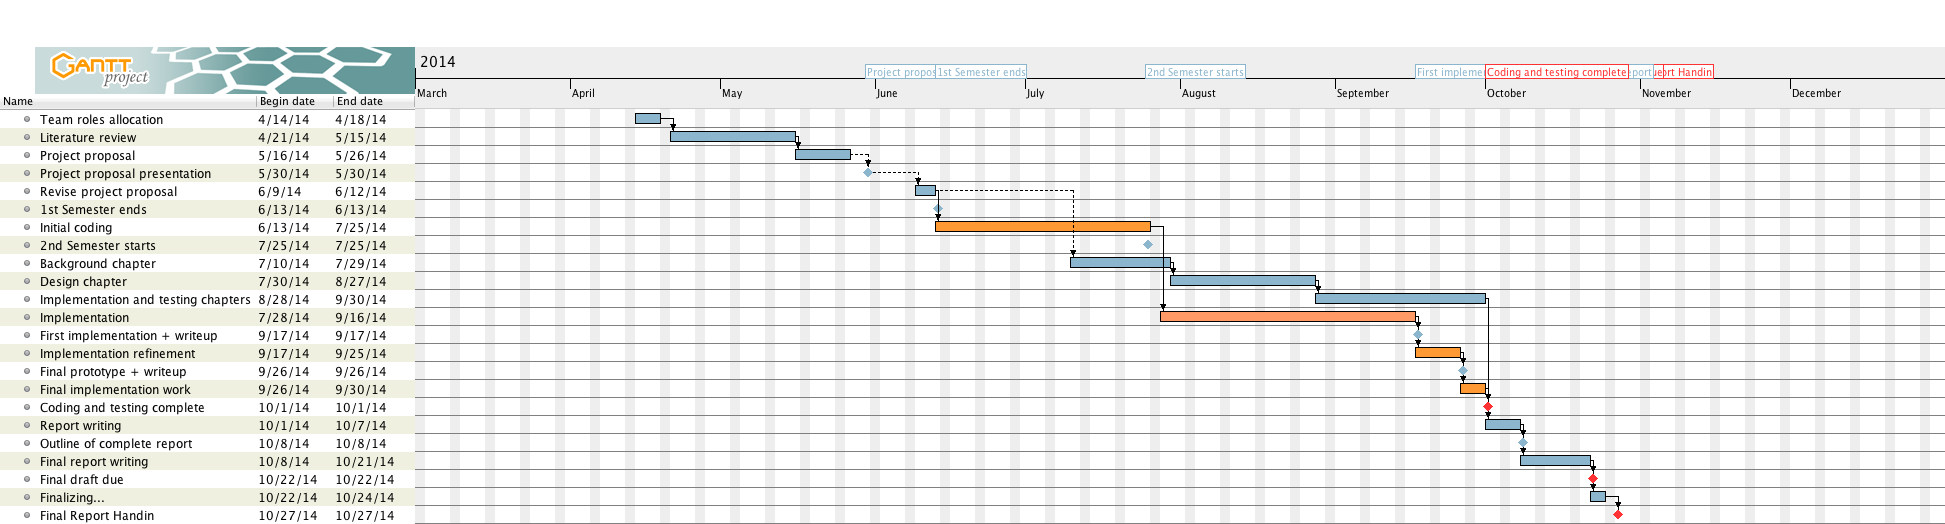
\includegraphics[width=\linewidth]{ganttchart}
\end{figure}
\end{landscape}
%}

\end{document}
